\documentclass[tikz,border=8pt]{standalone}
% Shared look for every TikZ diagram. Load with % Shared look for every TikZ diagram. Load with % Shared look for every TikZ diagram. Load with \input{../../tools/tikz-style.tex}
\usepackage[T1]{fontenc}
\usepackage{lmodern}
\renewcommand{\sfdefault}{lmr}  % diagrams use the same serif as the text
\usetikzlibrary{arrows.meta, positioning, shapes.geometric, calc, fit, backgrounds}
\definecolor{cblue}{HTML}{4C78A8}
\definecolor{corange}{HTML}{F58518}
\definecolor{cgreen}{HTML}{54A24B}
\definecolor{cred}{HTML}{E45756}
\definecolor{cpurple}{HTML}{B279A2}
\definecolor{cgrey}{HTML}{6B6B6B}
\tikzset{
  every picture/.style={font=\sffamily, line width=1.2pt},
  box/.style={draw=#1, fill=#1!12, rounded corners=4pt, align=center, inner sep=7pt, minimum height=1.1cm},
  box/.default=cgrey,
  arrow/.style={-{Stealth[length=3mm]}, draw=cgrey, line width=1.4pt},
  title/.style={font=\sffamily\bfseries\Large},
  note/.style={font=\sffamily\small, text=cgrey, align=center},
}
\AtBeginDocument{\hyphenpenalty=10000 \exhyphenpenalty=10000}

\usepackage[T1]{fontenc}
\usepackage{lmodern}
\renewcommand{\sfdefault}{lmr}  % diagrams use the same serif as the text
\usetikzlibrary{arrows.meta, positioning, shapes.geometric, calc, fit, backgrounds}
\definecolor{cblue}{HTML}{4C78A8}
\definecolor{corange}{HTML}{F58518}
\definecolor{cgreen}{HTML}{54A24B}
\definecolor{cred}{HTML}{E45756}
\definecolor{cpurple}{HTML}{B279A2}
\definecolor{cgrey}{HTML}{6B6B6B}
\tikzset{
  every picture/.style={font=\sffamily, line width=1.2pt},
  box/.style={draw=#1, fill=#1!12, rounded corners=4pt, align=center, inner sep=7pt, minimum height=1.1cm},
  box/.default=cgrey,
  arrow/.style={-{Stealth[length=3mm]}, draw=cgrey, line width=1.4pt},
  title/.style={font=\sffamily\bfseries\Large},
  note/.style={font=\sffamily\small, text=cgrey, align=center},
}
\AtBeginDocument{\hyphenpenalty=10000 \exhyphenpenalty=10000}

\usepackage[T1]{fontenc}
\usepackage{lmodern}
\renewcommand{\sfdefault}{lmr}  % diagrams use the same serif as the text
\usetikzlibrary{arrows.meta, positioning, shapes.geometric, calc, fit, backgrounds}
\definecolor{cblue}{HTML}{4C78A8}
\definecolor{corange}{HTML}{F58518}
\definecolor{cgreen}{HTML}{54A24B}
\definecolor{cred}{HTML}{E45756}
\definecolor{cpurple}{HTML}{B279A2}
\definecolor{cgrey}{HTML}{6B6B6B}
\tikzset{
  every picture/.style={font=\sffamily, line width=1.2pt},
  box/.style={draw=#1, fill=#1!12, rounded corners=4pt, align=center, inner sep=7pt, minimum height=1.1cm},
  box/.default=cgrey,
  arrow/.style={-{Stealth[length=3mm]}, draw=cgrey, line width=1.4pt},
  title/.style={font=\sffamily\bfseries\Large},
  note/.style={font=\sffamily\small, text=cgrey, align=center},
}
\AtBeginDocument{\hyphenpenalty=10000 \exhyphenpenalty=10000}

\begin{document}
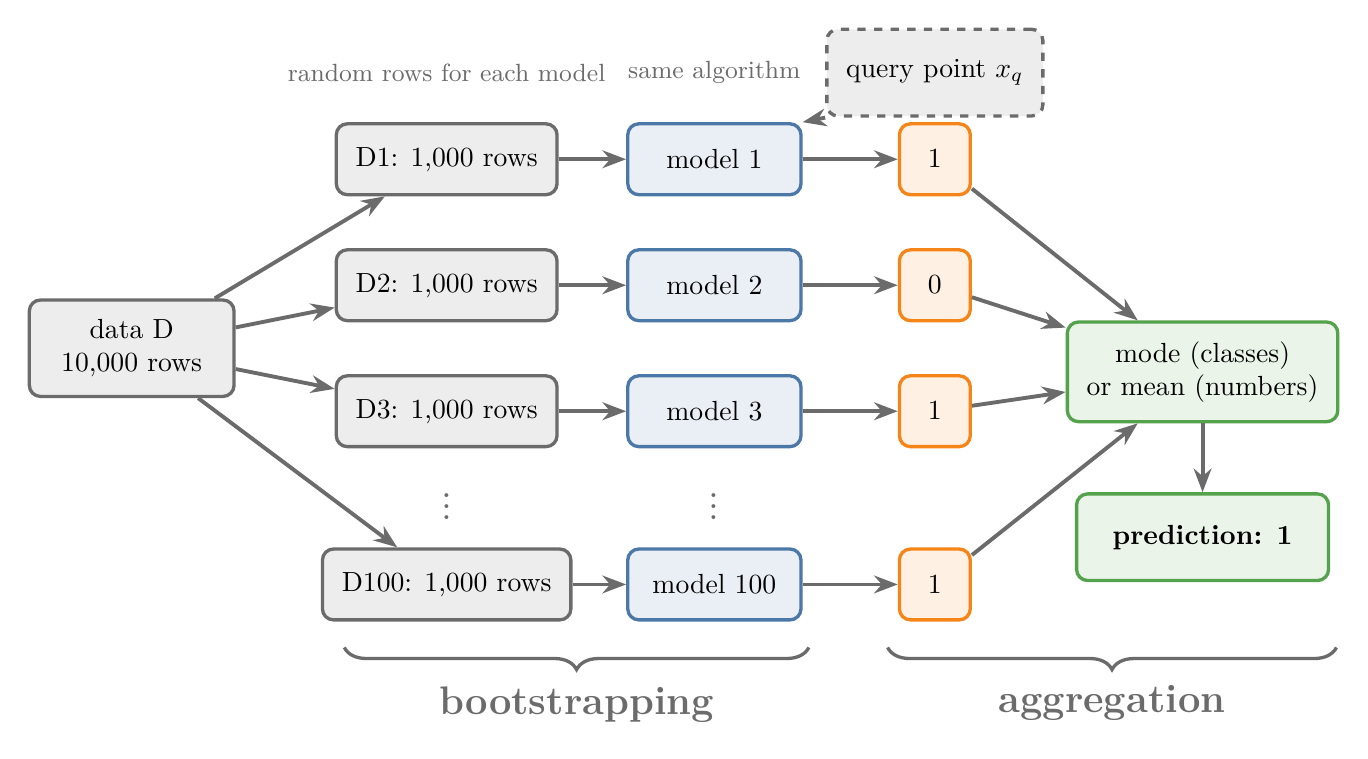
\begin{tikzpicture}[
  d/.style={box=cgrey, minimum width=2.6cm},
  s/.style={box=cgrey, minimum width=2.4cm, minimum height=0.9cm},
  m/.style={box=cblue, minimum width=2.2cm, minimum height=0.9cm},
  p/.style={box=corange, minimum width=0.9cm, minimum height=0.9cm},
  o/.style={box=cgreen, minimum width=3.2cm}]
  \node[d] (D) at (0,0) {data D\\10,000 rows};
  \foreach \i/\y/\lab in {1/2.4/D1, 2/0.8/D2, 3/-0.8/D3} {
    \node[s] (s\i) at (4,\y) {\lab: 1,000 rows};
    \node[m] (m\i) at (7.4,\y) {model \i};
    \draw[arrow] (D) -- (s\i); \draw[arrow] (s\i) -- (m\i);
  }
  \node[cgrey, font=\sffamily\Large] at (4,-1.9) {$\vdots$};
  \node[cgrey, font=\sffamily\Large] at (7.4,-1.9) {$\vdots$};
  \node[s] (s4) at (4,-3.0) {D100: 1,000 rows};
  \node[m] (m4) at (7.4,-3.0) {model 100};
  \draw[arrow] (D) -- (s4); \draw[arrow] (s4) -- (m4);
  \foreach \i/\v in {1/1, 2/0, 3/1, 4/1} {\node[p] (p\i) at (10.2,0 |- m\i) {\v}; \draw[arrow] (m\i) -- (p\i);}
  \node[o] (agg) at (13.6,-0.3) {mode (classes)\\or mean (numbers)};
  \foreach \i in {1,2,3,4} \draw[arrow] (p\i) -- (agg);
  \node[o, font=\sffamily\bfseries] (out) at (13.6,-2.4) {prediction: 1};
  \draw[arrow] (agg) -- (out);
  % phase braces
  \draw[decorate, decoration={brace, amplitude=8pt, mirror}, cgrey, line width=1.2pt] (2.7,-3.8) -- (8.6,-3.8)
     node[midway, below=10pt, title] {bootstrapping};
  \draw[decorate, decoration={brace, amplitude=8pt, mirror}, cgrey, line width=1.2pt] (9.6,-3.8) -- (15.3,-3.8)
     node[midway, below=10pt, title] {aggregation};
  \node[note] at (4,3.5) {random rows for each model};
  \node[note] at (7.4,3.5) {same algorithm};
  \node[d, dashed] (q) at (10.2,3.5) {query point $x_q$};
  \draw[arrow, dashed] (q.south west) -- (m1.north east);
\end{tikzpicture}
\end{document}
